\documentclass{article}

\usepackage{booktabs}
\usepackage{tabularx}
\usepackage{hyperref}
\usepackage[letterpaper, portrait, margin=1in]{geometry}

\usepackage[round]{natbib}

\usepackage{longtable}
\usepackage{xcolor}
\usepackage{blindtext}
\usepackage{enumitem}

\usepackage{array,multirow,graphicx}
\usepackage{float}
\usepackage{pdflscape}
\usepackage{lipsum} 
\usepackage{enumitem}
\usepackage{tikz}
\usepackage[hang,small]{caption}
\usetikzlibrary{positioning, shapes.geometric}
\newcommand{\tabitem}{~~\llap{\textbullet}~~}

\newcounter{hazard}
\newcommand{\showmycounter}{\stepcounter{hazard}\thehazard}

\hypersetup{
    colorlinks=true,       % false: boxed links; true: colored links
    linkcolor=red,          % color of internal links (change box color with linkbordercolor)
    citecolor=green,        % color of links to bibliography
    filecolor=magenta,      % color of file links
    urlcolor=cyan           % color of external links
}

% Test

\title{Hazard Analysis\\\progname}

\author{\authname}

\date{}

\newcommand{\lips}{\textit{Insert your content here.}}

\input{../Comments}
%% Common Parts

\newcommand{\progname}{Software Engineering} % PUT YOUR PROGRAM NAME HERE
\newcommand{\authname}{\textbf{Team 6, EcoOptimizers} \\
  \\ Nivetha Kuruparan
  \\ Sevhena Walker
  \\ Tanveer Brar
  \\ Mya Hussain
\\ Ayushi Amin} % AUTHOR NAMES

\usepackage{hyperref}
\hypersetup{colorlinks=true, linkcolor=blue, citecolor=blue, filecolor=blue,
urlcolor=blue, unicode=false}
\urlstyle{same}



\begin{document}

\maketitle
\thispagestyle{empty}

~\newpage

\pagenumbering{roman}

\begin{table}[hp]
\caption{Revision History} \label{TblRevisionHistory}
\begin{tabularx}{\textwidth}{ll>{\raggedright\arraybackslash}X}
\toprule
\textbf{Date} & \textbf{Developer(s)} & \textbf{Change}\\
\midrule
25 October 2024 & All & Created initial revision of Hazard Analysis\\
29 December 2024 & Tanveer Brar & Updated critical assumptions based on peer review feedback\\
January 3rd, 2025 & Sevhena Walker & Added Symbolic Constants, clarified boundaries of system, expanded recommended actions for HZ-13, adjusted failure mode for HZ-15 \\
March 24th, 2025, & Sevhena Walker & Updated system boundary and components\\
\bottomrule
\end{tabularx}
\end{table}

~\newpage

\tableofcontents

~\newpage

\pagenumbering{arabic}



\section{Introduction}

\subsection{Problem Statement}
The Information and Communications Technology (ICT) sector is currently responsible
for approximately 2-4\% of global CO2 emissions, a figure projected to rise to 14\% 
by 2040 without intervention ~\citep{BelkhirAndElmeligi2018}. To align with broader 
economic sustainability goals, the ICT industry must reduce its CO2 emissions by 72\% 
by 2040 ~\citep{FreitagAndBernersLee2021}. Optimizing energy consumption in software 
systems is a complex task that cannot rely solely on software engineers, who often 
face strict deadlines and busy schedules. This creates a pressing need for supporting 
technologies that help automate this process. This project aims to develop a tool that 
applies automated refactoring techniques to optimize Python code for energy efficiency 
while preserving its original functionality. 

\subsection{Hazard Analysis Introduction}

A hazard is defined as a property or condition in the system, 
combined with a condition in the environment, that has the potential to cause harm 
or damage—referred to as loss ~\citep{Leveson2021}. In software development, hazards can take various 
forms beyond just safety hazards, including security risks, usability challenges, 
incorrect inputs, or technical limitations like lack of internet connectivity.
\\

This project focuses on developing an automated tool to refactor Python code 
for energy efficiency while preserving its original functionality. While this 
initiative holds significant potential for reducing CO2 emissions in the 
Information and Communications Technology (ICT) sector, it also introduces 
various hazards. These hazards could arise from technical shortcomings, ethical 
challenges, or the inadvertent introduction of new problems during the refactoring 
process. This hazard analysis aims to identify and assess these risks to ensure 
the successful development and adoption of the tool.

\section{Scope and Purpose of Hazard Analysis}

The scope of this hazard analysis covers the potential risks and losses associated 
with the automated refactoring tool throughout its lifecycle. The primary hazards include:

\begin{itemize}

    \item \textbf{Technical Failures}: Inaccurate refactorings, undetected code 
    smells, or energy optimization that does not meet its intended goals could 
    result in performance issues or loss of functionality. 

    \item \textbf{Security Risks}: The automated nature of the tool may introduce 
    security vulnerabilities, particularly if the refactorings unintentionally 
    affect the security posture of the original code.

    \item \textbf{User Insensitivity}: If the tool is not designed with the users 
    in mind, it could disrupt developer workflows or lead to the rejection of the 
    tool. This can result in loss of productivity or missed opportunities for 
    energy efficiency.

    \item \textbf{External Conditions}: The tool’s dependency on environmental 
    factors, such as the availability of internet connection or access to 
    third-party libraries, could limit its usefulness in certain scenarios. 
    This can lead to delays or failures in the refactoring process.

\end{itemize}

The purpose of this analysis is to identify these hazards, assess their potential 
impact, and outline strategies for mitigating them. By doing so, we aim to prevent 
losses related to time, resources, security, and the overall effectiveness of the 
tool, ensuring that it contributes positively to reducing the ICT sector's energy 
consumption and CO2 emissions.

\section{System Boundaries and Components}

The system consists of three core modules integrated through a Visual Studio Code extension that serves as the primary user interface. All components operate locally on the user's machine without external dependencies.

\subsection{Core Modules}

\subsubsection{Analysis Module}
\begin{itemize}
    \item \textbf{Purpose}: Statically analyzes entire Python files to detect energy-inefficient code patterns
    \item \textbf{Key Functions}:
    \begin{itemize}
        \item Implements smell detection per requirement FR-2
        \item Outputs detection results
    \end{itemize}
    \item \textbf{Integration}: Receives complete files and smell configuration from VS Code extension
\end{itemize}

\subsubsection{Refactoring Module}
\begin{itemize}
    \item \textbf{Purpose}: Applies energy-saving transformations to address detected inefficiencies
    \item \textbf{Key Functions}:
    \begin{itemize}
        \item Generates refactored code versions per requirement FR-3
        \item Coordinates with Energy Measurement Module
        \item Outputs refactored code and energy metrics
    \end{itemize}
\end{itemize}

\subsubsection{Energy Measurement Module}
\begin{itemize}
    \item \textbf{Purpose}: Quantifies energy consumption using \texttt{codecarbon}
    \item \textbf{Key Functions}:
    \begin{itemize}
        \item Measures original and refactored code energy use
    \end{itemize}
\end{itemize}

\subsection{Visual Studio Code Extension}
\begin{itemize}
    \item \textbf{Role}: Primary user interface and system orchestrator
    \item \textbf{Key Functions}:
    \begin{itemize}
        \item Receives complete Python files from user workspace
        \item Displays detected smells with configurable visuals (FR-12)
        \item Allows triggering of refactoring operations (FR-16)
        \item Presents side-by-side refactoring comparisons (LFR-AP 1)
        \item Allows accept/reject decisions for changes (FR-16)
        \item Displays energy metrics and savings (FR-6)
    \end{itemize}
\end{itemize}

\begin{figure}[h]
    \centering
    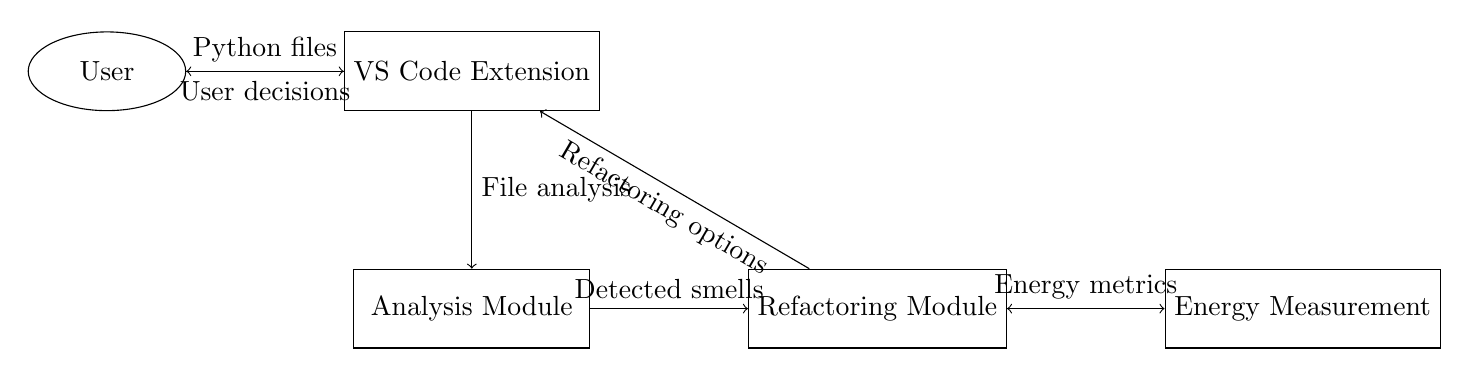
\begin{tikzpicture}[
        node distance=2cm,
        module/.style={rectangle, draw, minimum width=3cm, minimum height=1cm, text centered},
        user/.style={ellipse, draw, minimum width=2cm, minimum height=1cm}
    ]
        % Nodes
        \node (user) [user] {User};
        \node (extension) [module, right=of user] {VS Code Extension};
        \node (analysis) [module, below=of extension] {Analysis Module};
        \node (refactoring) [module, right=of analysis] {Refactoring Module};
        \node (energy) [module, right=of refactoring] {Energy Measurement};
        
        % Arrows
        \draw [->] (user) -- node[above] {Python files} (extension);
        \draw [->] (extension) -- node[right] {File analysis} (analysis);
        \draw [->] (analysis) -- node[above] {Detected smells} (refactoring);
        \draw [<->] (refactoring) -- node[above] {Energy metrics} (energy);
        \draw [->] (refactoring) -- node[below, sloped] {Refactoring options} (extension);
        \draw [->] (extension) -- node[below] {User decisions} (user);
    \end{tikzpicture}
    \caption{System component interaction diagram showing communication pathways}
    \label{fig:component-interaction}
\end{figure}

\section{Critical Assumptions}

\begin{itemize}
    \item The Energy Measurement Model will provide accurate and consistent energy consumption metrics across different platforms (Windows, macOS, Linux). There are no discrepancies in measurements due to platform differences that could result in ineffective refactoring.
    \item The Testing Module is provided with automated tests that include unit tests for core functionalities, integration tests for module interactions and edge case validations. There is no validation for minimum code coverage as it is decided by the user based on their needs and application complexity, but it is assumed that the provided tests effectively test all core functionalities to detect post refactoring bugs and regressions.
    \item The Refactoring Module solely identifies code smells that are validated by the development team's testing to reduce energy consumption. The module will not refactor the code smell if it is determined that the change will not result in measurable energy savings for the specific code being refactored.
    \item Custom-made refactoring strategies and Rope are capable of generating effective and correct refactoring.
    \item Sufficient data sets are available for the reinforcement learning model to provide increasingly accurate and efficient refactoring suggestions over time.
    \item GitHub Actions, which is a third-party dependency for the DevOps integration, is not suspended for a prolonged period of time.
    \item Users of the tool are experienced Python developers with knowledge of code refactoring and software optimization. Basic proficiency in programming is expected to navigate the tool and its features effectively.
    \item The tool will be used in a development environment, such as individual developer machines or a non-production remote repository, where configurations can be adjusted as needed. Stability and scalability requirements for large-scale production use are not assumed.
    \item The tool assumes that users act in good faith and use the system as intended. Potential hazards from malicious misuse (for example, injecting harmful code or exploiting refactoring logic) are considered out of scope for the current version but may be addressed in future versions.
    \item The tool assumes limited concurrent usage during energy measurement operation as simultaneous execution of resource-intensive processes could impact energy consumption metrics.
\end{itemize}

\newgeometry{margin=1.5cm}

\begin{landscape}
    % \clearpage
    % \thispagestyle{empty}
    % \pagenumbering{gobble}

    \section{Failure Mode and Effect Analysis}
    \centering
    \renewcommand{\arraystretch}{1.5}
    \setlength\LTleft{0pt}
    \setlength\LTright{0pt}
    \begin{longtable}{|
        >{\centering\arraybackslash}p{0.6cm}|
        >{\raggedright\arraybackslash}p{4cm}
        >{\raggedright\arraybackslash}p{4cm}
        >{\raggedright\arraybackslash}p{4cm}
        >{\raggedright\arraybackslash}p{4.7cm}
        >{\centering\arraybackslash}p{1.3cm}
        >{\centering\arraybackslash}p{1cm}|}
    \caption{FMEA Table}\\\hline
    \toprule \multicolumn{1}{|c}{\textbf{Component}} & \multicolumn{1}{c}{\textbf{Failure Modes}} & \multicolumn{1}{c}{\textbf{Effects of Failure}} & \multicolumn{1}{c}{\textbf{Causes of Failure}} & \multicolumn{1}{c}{\textbf{Recommended Action}} & \multicolumn{1}{c}{\textbf{SR}} & \multicolumn{1}{c|}{\textbf{Ref}}\\\hline
    \endhead
    \hline
    \multicolumn{7}{|r|}{\textit{Table continues on next page}}\\\hline
    \endfoot
    \bottomrule
    \endlastfoot
    
    \midrule
    \multicolumn{1}{|c|}{\multirow{10}{*}{\rotatebox[origin=c]{90}{\textbf{Energy Measurement}}}} 
    & Background tasks could be incorrectly included in energy measurement. & 
    Background tasks that are not related to the Python code under refactoring could skew the overall result for consumed energy. This could: \begin{itemize}[wide=0pt]
        \item skew the energy consumption metrics and mislead users. 
        \item produces refactorings that do not save energy due to faulty measurement. 
    \end{itemize} & The Energy Measurement Module lacks a filtering mechanism to isolate the specific Python code snippet being refactored. This allows unrelated background tasks or idle processes to be included in the overall energy measurement. & Use process-level tracking to distinguish between the Python code under refactoring and unrelated background tasks. & SCR-1 & HZ \showmycounter \\ \cline{2-7}
    
    \multicolumn{1}{|c|}{\multirow{18}{*}{\rotatebox[origin=c]{90}{\textbf{Energy Measurement}}}} & The Energy Measurement Module does not provide energy consumption data in a timely manner & \begin{itemize}[wide=0pt]
        \item User experiences delays in receiving energy consumption feedback, which can slow down their refactoring process.
        \item The tool may be considered inefficient by users, potentially causing them to not adopt it. 
    \end{itemize} & \begin{itemize}[wide=0pt]
        \item Computational overhead in the Energy Measurement Module
        \item Delays in accessing low level hardware components that are needed for energy measurement
    \end{itemize} & \begin{itemize}[wide=0pt]
        \item Investigate PyJoules' configuration options to find a balance between accuracy and performance based on the size and complexity of the code being refactored. 
        \item Implement parallel processing to measure energy consumption and run code smell detection simultaneously. This can reduce the overall time by allowing energy measurements to be done without holding up other tasks.
        \item Implement a graceful timeout mechanism if PyJoules takes too long to respond. 
        \item Provide users with an estimated time for completion so they are aware of ongoing measurements if energy measurement exceeds a set time. 
    \end{itemize} & SCR-1, SCR-10 & HZ \showmycounter \\
    
    \multicolumn{1}{|c|}{\multirow{13}{*}{\rotatebox[origin=c]{90}{\textbf{Energy Measurement}}}} & The energy measure module does not provide any data at all & Refactoring fails due to no energy metrics available for validation of changes & \begin{itemize}[wide=0pt]
        \item The system does not have the necessary administrative or system-level permissions to access energy-related data, especially in cloud environments
        \item The energy measurement process might be too slow, resulting in timeouts or delays that cause no metrics to be reported within the expected time frame.
    \end{itemize} & \begin{itemize}[wide=0pt]
        \item Ensure the software has sufficient permissions to access low-level system metrics, such as power usage, and grant administrative privileges if needed.
        \item Increase the allowed time frame for measurements to complete
        \item Implement a functionality in the system that allows that prompts the user with a request to pause the refactoring process and restart at the same point when the system is less busy
    \end{itemize} & SCR-1, SCR-3, SCR-10 & HZ \showmycounter \\ \cline{2-7}

    \hline

    \multicolumn{1}{|c|}{\multirow{11}{*}{\rotatebox[origin=c]{90}{\textbf{Testing}}}} & Test not able to run due to refactoring &
    \begin{itemize}[wide=0pt]
        \item Testing coverage not met
        \item Unable to test business logic of user code
        \item Unable to complete refactorings
    \end{itemize}
    & Test cases dependent on some modules that have been refactored &
    \begin{itemize}[wide=0pt]
        \item Use AST as a base for testing
        \item Ensure that any refactorings that involve variable, class or function name changes are disabled on default and require explicit enabling from the user
    \end{itemize}
    & SCR-2 & HZ \showmycounter \\ \cline{2-7}
    
    & Provided test suite misses critical scenarios& 
    \begin{itemize}[wide=0pt]
        \item The refactored code could fail in production under specific conditions, leading to potential downtime or incorrect behaviour.
    \end{itemize} &
    \begin{itemize}[wide=0pt]
        \item  Limited test suite or lack of coverage for particular scenarios.
    \end{itemize}
    & Implement syntactical analysis in refactoring to mitigate code functionality changes & SCR-2 & HZ \showmycounter \\ \cline{2-7}
    
    \hline

    \multicolumn{1}{|c|}{\multirow{20}{*}{\rotatebox[origin=c]{90}{\textbf{Refactoring}}}} & Incorrect refactorings suggestions were given & 
    \begin{itemize}[wide=0pt]
        \item Refactored code increases the energy consumption instead of reducing it.
        \item Functionality of refactored code is not consistent from that of the original code.
    \end{itemize} &
    \begin{itemize}[wide=0pt]
        \item Inadequate training of the reinforcement learning model. 
        \item Refactoring logic misses some edge cases. 
        \item Reinforcement learning model creates syntactically incorrect code. 
    \end{itemize}
        & Validate the changes by verifying energy consumption statistics before applying changes to the code by adding validation rules & SCR-2 & HZ \showmycounter \\ \cline{2-7}
        
    & A memory leak occurs during the refactoring process & 
    \begin{itemize}[wide=0pt]
        \item Gradual increase in memory usage leading to application lagging, crashing or freezing
    \end{itemize} &
    \begin{itemize}[wide=0pt]
        \item  Poor memory management during the refactoring process
    \end{itemize}
    & Implement automatic garbage collection or memory de-allocation after each refactoring step & SCR-8 & HZ \showmycounter \\ \cline{2-7}
    
    & Unable to revert refactorings & 
    \begin{itemize}[wide=0pt]
        \item User loses confidence in integrity of system
        \item Unable to pick which refactorings to keep and which to discard based on user input
    \end{itemize} &
    \begin{itemize}[wide=0pt]
        \item  Faulty version control strategy
    \end{itemize}
    & Implement a robust version control system that follows a granular commit system tracking each change with precision & SCR-4 & HZ \showmycounter \\ \cline{2-7}
    
    
    & The refactoring improves energy efficiency but degrades other performance metrics like speed or memory usage & 
    \begin{itemize}[wide=0pt]
        \item The software becomes slower or uses more memory, which could counteract the benefits of energy optimization.
    \end{itemize} &
    \begin{itemize}[wide=0pt]
        \item Poor trade-offs made by the refactoring algorithm between energy efficiency and other performance factors.
    \end{itemize}
    & Implement multifactor optimization, balancing energy efficiency with other performance metrics. If this is not possible inform the user of potential degradation when suggesting at-risk refactorings. & SCR-2 & HZ \showmycounter \\

    \multicolumn{1}{|c|}{\multirow{13}{*}{\rotatebox[origin=c]{90}{\textbf{Refactoring}}}}& The refactoring tool modifies code that relies on external libraries, causing incompatibility with these libraries. & 
    \begin{itemize}[wide=0pt]
        \item Code fails to execute or produces unexpected behaviour due to altered interactions with third-party libraries.
    \end{itemize} &
    \begin{itemize}[wide=0pt]
        \item Lack of awareness of how certain refactorings impact external dependencies, especially with complex or dynamically loaded libraries.
    \end{itemize}
    & Implement a detection mechanism that identifies external library dependencies and exempts them from refactorings unless explicitly requested by the user. & SCR-5 & HZ \showmycounter \\ \cline{2-7}

    & The tool accesses or refactors code that contains sensitive information (e.g., API keys, credentials), which could lead to unintentional exposure or mismanagement of this data. & 
    \begin{itemize}[wide=0pt]
        \item Sensitive information could be mishandled, leading to potential security breaches, privacy violations, or unauthorized access.
    \end{itemize} &
    \begin{itemize}[wide=0pt]
        \item Refactorings alter or expose parts of the code that store or transmit sensitive data, without proper checks.
    \end{itemize}
    & Implement security-focused static analysis tools that identify sensitive code sections and prevent them from being refactored. Warn users when refactoring such areas. & SCR-6 & HZ \showmycounter \\ \hline 

    
    \multicolumn{1}{|c|}{\rotatebox[origin=c]{90}{\parbox{4cm}{\begin{center}\textbf{Reinforcement} \\ \textbf{Learning}\end{center}}}} & Model overfitting & Less effective when applied to unseen or more diverse codebases resulting in suboptimal and/or incorrect refactorings for new projects. & \begin{itemize}[wide=0pt]
        \item Over-training model on similar datasets
    \end{itemize} & Use a diverse and representative dataset for training the model & SCR-7 & HZ \showmycounter \\ \cline{2-7}

    
    \multicolumn{1}{|c|}{\multirow{22}{*}{\rotatebox[origin=c]{90}{\textbf{Reinforcement Learning}}}} & Bias in recommendations & Model starts favouring certain types of refactorings or ignoring others that could be more efficient for different scenarios. & \begin{itemize}[wide=0pt]
        \item Imbalanced reward function
        \item Not enough exploration actions done by the model
        \item Unrealistic straining data simulations used
    \end{itemize} &
    \begin{itemize}[wide=0pt]
        \item The model should be regularly audited for bias. The audit should determine that the model chooses the most efficient refactoring \& is constantly proposing new solutions to learn from.
        \item Ensure that the model's training data is not biased towards any particular refactoring and/or code pattern. There should an equal (or near equal as possible) emphasis put on each separate category of data.
        \item Regularly retrain the model.
    \end{itemize}
    & SCR-7 & HZ \showmycounter \\ \cline{2-7}

    
    & Model drift and degradation & The RL model becomes less effective over time due to changes in code styles, and best practices, or the introduction of new refactoring strategies leading to a degradation in performance and accuracy of refactoring suggestions. & Passing of time and evolution of software practices &
    \begin{itemize}[wide=0pt]
        \item Regularly retrain the model using up-to-date data and monitor its performance to detect signs of drift.
        \item Implement a feedback loop to incorporate user corrections into the training data.
    \end{itemize}
    & SCR-7 & HZ \showmycounter \\ \cline{2-7}

    
    & Model generates suboptimal or erroneous refactorings. & 
    \begin{itemize}[wide=0pt]
        \item Incorrect or harmful refactorings are applied without proper oversight, leading to system instability.
    \end{itemize} &
    \begin{itemize}[wide=0pt]
        \item Over-reliance on automated suggestions without sufficient human review or fail-safes.
    \end{itemize}
    & Require human approval for significant refactorings or apply thresholds to reject low-confidence suggestions from the model. & SCR-9 & HZ \showmycounter \\ \cline{2-7}\hline


    \multicolumn{1}{|c|}{\multirow{20}{*}{\rotatebox[origin=c]{90}{\textbf{Reinforcement Learning \& Energy Measurement}}}} &  Incorrect energy measurements are used for refactoring decisions, leading to poor optimization or functional errors in the refactored code. & 
    \begin{itemize}[wide=0pt]
        \item Incorrect energy measurements leading to suboptimal or erroneous refactoring decisions.
        \item Energy inefficiencies or functional degradation in the refactored code
    \end{itemize} & Incorrect measurements of energy usage was validated and used by Reinforcement Learning Model which created incorrect refactorings. & Introduce validation mechanisms for energy data before using it for refactoring decisions. & SCR-1 & HZ \showmycounter \\ \cline{2-7}


    & Failed tests result in incorrect data being used for model training, causing the reinforcement learning model to learn from inaccurate or irrelevant data. & 
    \begin{itemize}[wide=0pt]
        \item Test failures causing incorrect updates to the learning model's training data
        \item Reinforcement learning model learns from incorrect outcomes, reducing its effectiveness
    \end{itemize} &
    \begin{itemize}[wide=0pt]
        \item Failed test cases are not handled sufficiently during model training.
    \end{itemize}
    & Implement safeguards to exclude failed test cases from training data or tag them for further analysis. & SCR-7, SCR-12 & HZ \showmycounter \\ \cline{2-7} 


    & Simultaneous refactoring operations without proper synchronization lead to conflicts or inconsistencies, causing code instability or unexpected behavior. & 
    \begin{itemize}[wide=0pt]
        \item Conflicts or inconsistencies arising from multiple refactoring operations executed simultaneously
        \item Code instability or unintended behavior in the refactored codebase
    \end{itemize} &
    \begin{itemize}[wide=0pt]
        \item Lack of synchronization or conflict resolution mechanisms for parallel refactoring
    \end{itemize}
    & Introduce locking mechanisms or dependency checks to ensure safe concurrent operations. & SCR-13 & HZ \showmycounter \\ \hline

    \multicolumn{1}{|c|}{\multirow{12}{*}{\rotatebox[origin=c]{90}{\textbf{All Components}}}} & The system shuts down or crashes during an ongoing optimization process. &
    \begin{itemize}[wide=0pt]\item Energy Measurement: Incomplete energy metrics can result in inaccurate energy savings reporting. \item Refactoring: Loss of progress in ongoing optimization can lead to delays.  \item Reinforcement Learning: Loss of training data generated during the session can reduce the model's ability to improve optimization recommendations over time. \end{itemize} &
    \begin{itemize}[wide=0pt] \item Hardware failure, power outage or insufficient system resources \item Unhandled software exceptions or errors during the tool's usage \item Prolonged measurement operations that exceed system capacity \end{itemize} &
    \begin{itemize}[wide=0pt] \item Implement a checkpointing mechanism to periodically save intermediate refactoring states \item Enable a recovery workflow to reload saved checkpoints and resume from the last recorded state  \end{itemize} &
    SCR-1, SCR-4, SCR-14 &
    HZ-\showmycounter \\ \hline
\end{longtable}


\end{landscape}

\newgeometry{margin=1in}

\pagenumbering{arabic}


\section{Safety and Security Requirements}

\begin{table}[H]
    \centering
    \renewcommand{\arraystretch}{1.2}
    \begin{tabular}{|l|c|}
        \toprule \textbf{Symbol} & \textbf{Value} \\
        \midrule
        LOG\_THRESH & 100\% \\
        REFACTOR\_TEST\_THRESH & 100\% \\
        REFACTOR\_SECURE\_THRESH & 100\% \\
        REFACTOR\_EFFECT\_THRESH & 95\% \\
        PERFORM\_TOL & 5\% \\
        RUNS\_THRESH & 100\% \\
        EDIT\_THRESH & 100\% \\
        DETECT\_ACC & 100\% \\
        MEM\_ALERT\_THRESH & 100\% \\
        RISK\_REFACTOR\_THRESH & 100\% \\
        ENERGY\_DELAYS & 100\% \\
        ENERGY\_VALID\_THRESH & 100\% \\
        TEST\_TRIAGE\_THRESH & 100\% \\
        SAVE\_TIME & 30 sec \\
        MAX\_DATA\_LOSS & 1\% \\
        FAIL\_SCENARIO\_THRESH & 100\% \\
        \bottomrule
    \end{tabular}
    \caption{Symbolic Constants}
    \label{tab:sym}
\end{table}

\begin{enumerate}[label=SCR \arabic*., wide=0pt, leftmargin=*]

    \item \emph{The system shall log all energy consumption measurements with timestamps and indicate which processes were measured to aid in future analysis and troubleshooting.}\\
    {\bf Rationale:} Detailed logging with timestamps and process attribution ensures accurate energy data and helps identify delays or misattributions.\\
    {\bf Fit Criterion:} \texttt{LOG\_THRESH} of energy analysis logs must include timestamps and process-level breakdowns of all measured processes.\\
    {\bf Associated Hazards:} HZ-1, HZ-2, HZ-3, HZ-19\\
    {\bf Priority:} High

    \item \emph{The system shall ensure that all refactored code has comprehensive test coverage and passes performance metrics such as energy efficiency, speed, and memory usage.}\\
    {\bf Rationale:} Proper test coverage and performance checks prevent faulty code from being introduced and ensure refactorings improve or maintain performance.\\
    {\bf Fit Criterion:} \texttt{REFACTOR\_TEST\_THRESH} of refactorings must pass tests covering all code paths, and performance must remain within \texttt{PERFORM\_TOL} across energy, speed, and memory metrics.\\
    {\bf Associated Hazards:} HZ-4, HZ-5, HZ-6, HZ-9\\
    {\bf Priority:} High

    \item \emph{The system shall check for necessary system-level permissions to access energy consumption data and alert users if permissions are missing.}\\
    {\bf Rationale:} Lack of access may lead to failure in energy data retrieval, which can hinder the accuracy of analysis.\\
    {\bf Fit Criterion:} \texttt{RUNS\_THRESH} of runs shall check for and request permissions if required, and alert the user in case of failures.\\
    {\bf Associated Hazards:} HZ-3\\
    {\bf Priority:} High

    \item \emph{The system shall ensure version control for each refactoring, allowing changes to be reverted in case of errors.}\\
    {\bf Rationale:} Version control helps prevent loss of code or data and allows developers to revert refactorings if necessary.\\
    {\bf Fit Criterion:} \texttt{EDIT\_THRESH} of changes shall be recorded, allowing full reversion with no data loss.\\
    {\bf Associated Hazards:} HZ-8, HZ-19\\
    {\bf Priority:} High

    \item \emph{The system shall detect and exempt external library dependencies from refactorings to avoid compatibility issues.}\\
    {\bf Rationale:} Modifying external dependencies could lead to system instability or incompatibility with other tools or frameworks.\\
    {\bf Fit Criterion:} \texttt{DETECT\_ACC} detection accuracy for external library code during refactoring.\\
    {\bf Associated Hazards:} HZ-10\\
    {\bf Priority:} Medium

    \item \emph{The system shall not refactor or alter code containing sensitive information (noted by user), ensuring security is maintained.}\\
    {\bf Associated Rationale:} Refactoring sensitive code may introduce vulnerabilities and compromise security.\\
    {\bf Fit Criterion:} \texttt{REFACTOR\_SECURE\_THRESH} of refactorings must pass a security check to avoid tampering with sensitive information.\\
    {\bf Associated Hazards:} HZ-11\\
    {\bf Priority:} High

    \item \emph{The reinforcement learning model shall be trained on diverse datasets and periodically audited to avoid bias and prevent degradation.}\\
    {\bf Rationale:} Overfitting or model degradation can lead to suboptimal or biased refactorings, impacting the system's effectiveness.\\
    {\bf Fit Criterion:} \texttt{REFACTOR\_EFFECT\_THRESH} of refactorings should be equally effective across different types of projects, and model audits should occur at least quarterly.\\
    {\bf Associated Hazards:} HZ-12, HZ-13, HZ-14\\
    {\bf Priority:} Medium

    \item \emph{The system shall implement memory leak detection during refactoring and alert users if any issues are detected.}\\
    {\bf Rationale:} Memory leaks may cause system crashes and reduce performance.\\
    {\bf Fit Criterion:} \texttt{MEM\_ALERT\_THRESH} of memory leak incidents should trigger an error alert and resolution process.\\
    {\bf Associated Hazards:} HZ-7\\
    {\bf Priority:} Medium

    \item \emph{The system shall require user approval for high-impact refactorings (those modifying more than 50 lines of code) or low-confidence refactorings (based on a ranked list of code smells), providing visibility and oversight for critical changes.}\\
    {\bf Rationale:} Automated decisions could introduce errors without human oversight, and users should be aware of significant changes.\\
    {\bf Fit Criterion:} \texttt{RISK\_REFACTOR\_THRESH} of refactorings exceeding 50 lines or flagged as low-confidence by the ranked smell list must require user approval before proceeding.\\
    {\bf Associated Hazards:} HZ-15\\
    {\bf Priority:} High

    \item \emph{The system shall alert users to any delays or failures in reporting energy consumption, ensuring transparency in reporting.}\\
    {\bf Rationale:} Users need to be aware of any issues in energy reporting to troubleshoot and resolve potential problems.\\
    {\bf Fit Criterion:} \texttt{ENERGY\_DELAYS} of energy measurement delays or failures must trigger a user alert.\\
    {\bf Associated Hazards:} HZ-2, HZ-3\\
    {\bf Priority:} High

    \item \emph{The system shall validate energy measurement data before using it for refactoring decisions.}\\
    {\bf Rationale:} Incorrect energy measurements can lead to suboptimal or erroneous refactoring decisions, affecting code efficiency and functionality.\\
    {\bf Fit Criterion:} \texttt{ENERGY\_VALID\_THRESH} of energy measurement data shall be validated before use in refactoring, and invalid data shall be flagged and not used for optimization.\\
    {\bf Associated Hazards:} HZ-16\\
    {\bf Priority:} High

    \item \emph{The system shall ensure that failed test cases are excluded or flagged before being used in training the reinforcement learning model.}\\
    {\bf Rationale:} If test failures are used in training, the learning model may develop inaccurate or ineffective strategies, reducing its overall performance.\\
    {\bf Fit Criterion:} \texttt{TEST\_TRIAGE\_THRESH} of failed test cases shall be identified and excluded or flagged for further analysis during model training.\\
    {\bf Associated Hazards:} HZ-17\\
    {\bf Priority:} High

    \item \emph{The system shall implement synchronization mechanisms to prevent conflicts during concurrent refactorings, ensuring that refactoring operations do not interfere with each other.}\\
    {\bf Rationale:} Without synchronization, concurrent refactorings could lead to code instability, unintended behavior, or data corruption.\\
    {\bf Associated Hazards:} HZ-18\\
    {\bf Priority:} High

    \item \emph{The system shall implement a checkpointing mechanism to periodically save the state of the optimization process, including the refactoring progress, energy measurement data, and reinforcement learning model state, and provide recovery options in case of a system shutdown or failure.}\\
    {\bf Rationale:} Periodic checkpointing ensures progress is not lost during unexpected system failures, allowing users to resume optimization.\\
    {\bf Fit Criterion:} The system must save progress at least every \texttt{SAVE\_TIME} during optimization and allow recovery with no more than \texttt{MAX\_DATA\_LOSS} in \texttt{FAIL\_SCENARIO\_THRESH} of failure scenarios.\\
    {\bf Associated Hazards:} HZ-19\\
    {\bf Priority:} High

\end{enumerate}

\section{Roadmap}

Requirements that will be implemented during the capstone timeline:

\renewcommand{\arraystretch}{1.2}
\begin{tabular}{p{0.3\textwidth} p{0.3\textwidth} p{0.3\textwidth}}
    \begin{itemize}[wide=0pt]
        \item SCR 1
        \item SCR 2
        \item SCR 3
        \item SCR 4
    \end{itemize} &
    \begin{itemize}[wide=0pt]
        \item SCR 5
        \item SCR 6
        \item SCR 9
        \item SCR 10
    \end{itemize} &
    \begin{itemize}[wide=0pt]
        \item SCR 11
        \item SCR 12
        \item SCR 13
    \end{itemize} \\
\end{tabular}

\medskip

\noindent
Requirements implemented in the future:
\begin{itemize}
    \item SCR 7: This will be audited on a regular basis which will be a future implementation.
    \item SCR 8: This can be implemented in the future as it is not a high priority and not the biggest concern to this project.
\end{itemize}

\newpage{}

\section*{Appendix --- Reflection}

\subsubsection*{Nivetha Kuruparan}

\begin{enumerate}
  \item \textit{What went well while writing this deliverable?}
  
  While writing this hazard analysis, one thing that went well was identifying missing requirements that had not been captured in the original SRS document. As we analyzed potential hazards, especially related to security and communication, it became clear that certain protections—like secure authentication and making sure we are tracking the correct energy needed more attention. Catching these gaps allowed us to enhance the system's robustness and ensure that our requirements addressed both safety and security concerns comprehensively. This process also helped align our priorities more effectively, as we were able to associate risks with specific requirements and refine the overall design.

  \item \textit{What pain points did you experience during this deliverable, and how did you resolve them?}
  
  A pain point during this deliverable was mapping out the safety requirements to the identified hazards. It was challenging to ensure that each requirement accurately addressed specific risks, especially when certain hazards overlapped or required more nuanced handling. Determining the exact scope of each safety requirement, while avoiding redundancy, took considerable time and effort. To resolve this, we revisited the hazard analysis step-by-step, carefully analyzing each potential failure and its impact on the system, which helped clarify how the requirements should be structured. Collaborating with the team to cross-check each hazard also helped ensure that we didn’t overlook critical risks or assign incorrect priorities.

\end{enumerate}

\subsubsection*{Sevhena Walker}

\begin{enumerate}
  \item \textit{What went well while writing this deliverable?}
  
  One thing that went really well during the hazard analysis was how it helped me catch issues I’d originally missed. The structured process made it easier to step back and look at our project from a different perspective, which helped highlight potential risks I hadn’t thought of before. 

  \item \textit{What pain points did you experience during this deliverable, and how did you resolve them?}
  
  I'll be honest the worst part of this deliverable was formatting the FMEA table in latex. It doesn't seem right to talk about pain points without mentioning the one thing that truly had me pulling my hair out. In terms of the actual content of the deliverable, brainstorming hazards was challenging, but not exactly a pain. The challenging part was coming up with solution or mitigating actions to counter those hazards. Some components, like the reinforcement model, I have truly no experience with and its pretty hard to come up with solutions to risks you have never even experienced, let alone thought of. 
  
\end{enumerate}

\subsubsection*{Tanveer Brar}

\begin{enumerate}
    \item \textit{What went well while writing this deliverable?}

    This deliverable was pretty short compared to previous ones but we were still on top of our toes when it came to planning it within the team. I like that we allowed everyone to pick up topics that interested them the most and left the key piece of work(FMEA table) to be worked on collaboratively in Overleaf by everyone. Timely spiliting of the work gave us ample time to finish individual assignments as well as review other people's contributions.

    \item \textit{What pain points did you experience during this deliverable, and how did you resolve them?}

    The main challenge that I faced was mapping the Failure Modes to appropriate security requirements. Some of the failure modes that I came up with aligned with the security requirements written previously, but more content needed to be added to those. To resolve this, I added the additional description needed for these security requirements for some hazards and created new requirements for others.

\end{enumerate}

\subsubsection*{Mya Hussain}

\begin{enumerate}
  \item \textit{What went well while writing this deliverable?}
  
  We divided up the work early and were all able to complete sections at our own 
  pace or ahead of time depending on our midterm schedules. This week was 
  particularly busy because all of us had midterms so I was able to complete 
  my section during reading week to reduce the capstone workload during the week. 
  Although I will say it's a little disappointing that every time we are done on 
  time (which has been every time so far) the deliverable is extended last minute. 
  I don't want to complain too much though because I have a feeling that if I do 
  complain it won't be extended next time I'd actually like it to be. So far team 
  dynamics and morale have been good. I appreciate the level of organization we've 
  been able to have so far as it made collaborating so much smoother and has helped 
  everyone stay on track with our tasks.

  \item \textit{What pain points did you experience during this deliverable, and how did you resolve them?}
  
  Determining which factors qualify as hazards for our analysis was somewhat unclear.
  A hazard is defined as anything with the potential to cause harm or loss, yet certain    
  risks may emerge from poor design, complicating our decision on whether to include them.    
  For example, user interface hazards like "the tool does not provide clear feedback    
  to the user after refactoring" can technically be classified as a hazard. While we    
  aim to mitigate team-imposed hazards, it raises the question of whether we should    
  simply avoid designing a flawed product in the first place, and not include these    
  hazards in the analysis or if we should do a worst-case analysis and include every    
  possible pitfall. The same argument could be made for some security hazards for example    
  "while parsing user input code, the software encounters malware and executes it,"    
  avoiding this is something a good tool should already have built in, so it begs    
  the question of "how bad do we envision our final product when analyzing hazards?"    
  We were able to get some clarification on this in our TA 1-1 meeting but ultimately    
  tried to keep it high level so our report didn't end up being too long.

\end{enumerate}

\subsubsection*{Ayushi Amin}

\begin{enumerate}
  \item \textit{What went well while writing this deliverable?}
  
  I think one of the best things about writing this deliverable was how well we collaborated using Overleaf. It made it super easy to 
  work together on the FMEA table. We divided up the work, so everyone had their own sections to focus on, but we also helped each 
  other out when needed. This teamwork really made a difference because we could share ideas and give feedback in real time.
  Even though we had midterms this week, which delayed our progress a bit, everything ended up working out. We managed our time well, 
  and I was impressed with how we all stayed on track despite the busy schedule. It felt good to see how our combined efforts came 
  together in the final product. Overall, I think our collaboration really strengthened the quality of our work.

  \item \textit{What pain points did you experience during this deliverable, and how did you resolve them?}
  
  One big challenge I faced was figuring out the difference between general risks and specific hazards for our project. At first, it was 
  a bit confusing, and we spent some time debating whether certain issues were specific enough. To resolve this, I looked up examples from
  other projects, which helped clarify things for everyone. Overall, even though there were some bumps along the way, working through these 
  challenges taught me a lot about hazard analysis and teamwork in software development.
  
\end{enumerate}

\subsubsection*{Group Answer}

\begin{enumerate}
    \item[3.] \textit{Which of your listed risks had your team thought of before this deliverable, and which did you think of while doing this deliverable? For the latter ones (ones you thought of while doing the Hazard Analysis), how did they come about?}

    The risks that we had thought of before this deliverable include  HZ6, HZ7, HZ9 and HZ10. All remaining risks(HZ1, HZ2, HZ3, HZ4, HZ5, HZ8, HZ11, HZ12, HZ13, HZ14, HZ15 and HZ16) were thought of during the deliverable. To come up with ideas, we analyzed the system on a component by component basis in order to identify risks on a granular level(components defined earlier in Section 3 of this document).  Defining critical assumptions before brainstorming the risks helped create a boundary for lookout for possible things that could go wrong with each component. It is important to note that a deeper understanding of our dependencies, such as PyJoules for energy measurements, helped identify possible things that could go wrong when implementing those in their respective modules. We adopted an iterative approach to the brainstorming, as identifying ground level risks helped to identify other risks over an entire week of deliberation.

    \item[4.] \textit{Other than the risk of physical harm (some projects may not have any appreciable risks of this form),
    list at least 2 other types of risk in software products. Why are they important to consider?}

    \begin{enumerate}
        \item Data Security Risk: Software products are a storehouse of data related to its users. If sensitive data is exposed to vulnerabilities, it can leads to breaches. This risk is important to consider as a a breach can harm users as well as the organization’s reputation. Addressing this risk is critical for maintaining trust and preventing legal battles.
        \item Operational Risk: Live hosted software products are bound to face risks related to live performance, such as slow performance and/or system downtime. These are important to consider as they are post-implementation risks that directly impact system availability to users. This can impact user productivity and cause financial loss to the organization, which is why they should be considered.
    \end{enumerate}

\end{enumerate}

\bibliographystyle {plainnat}
\bibliography{../../refs/References}

\end{document}
